\documentclass{standalone}
\usepackage{tikz}
\usetikzlibrary{patterns, positioning}
\usepackage[sfdefault]{ClearSans} %% option 'sfdefault' activates Clear Sans as the default text font
\usepackage[T1]{fontenc}

\begin{document}
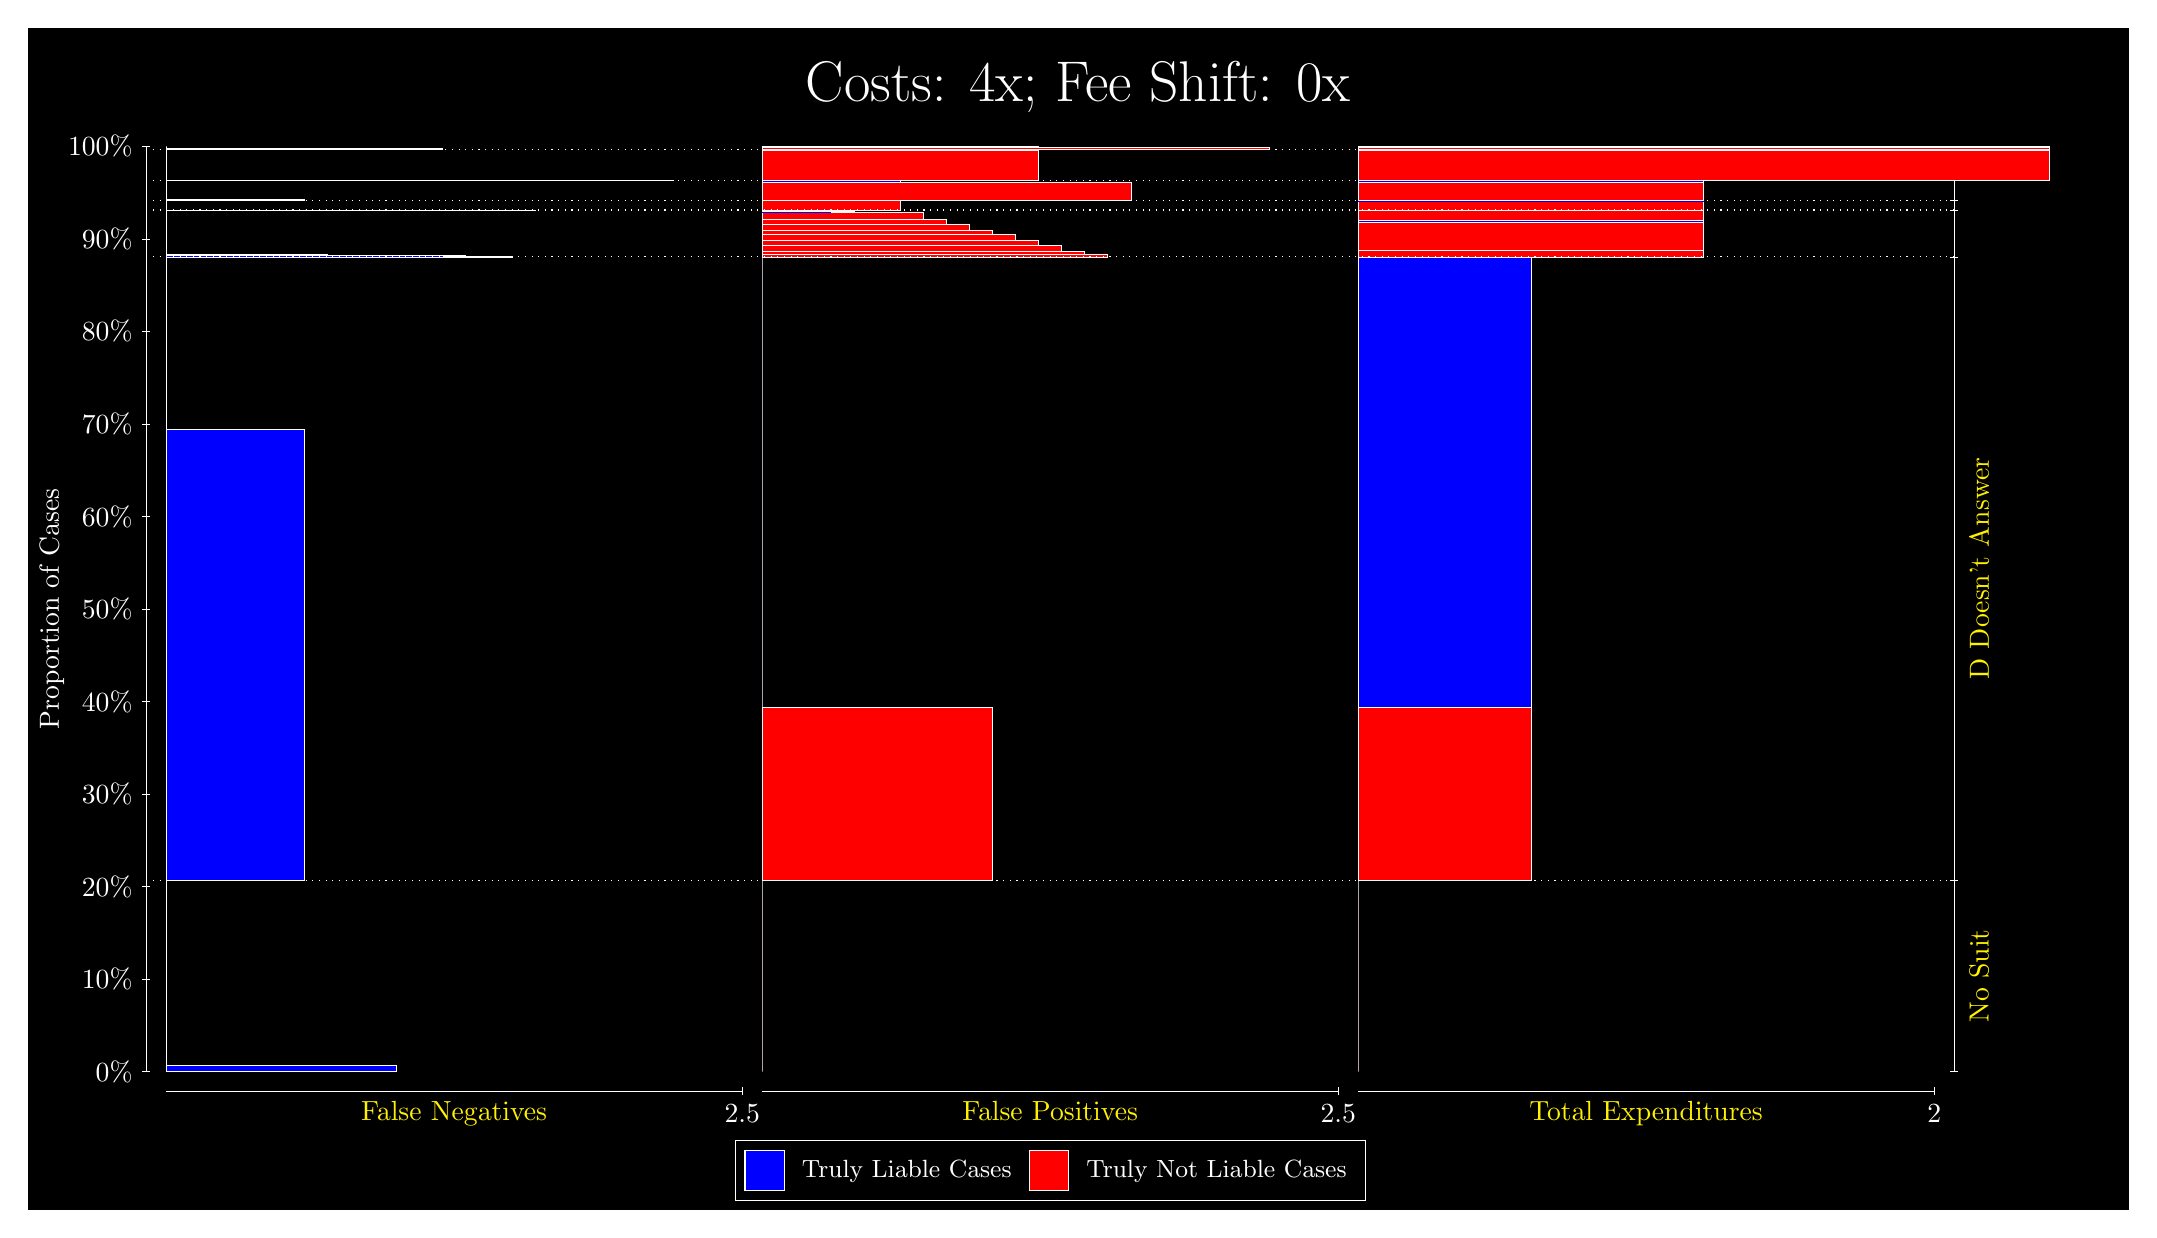
\begin{tikzpicture}
\draw[fill=black] (0,0) rectangle (26.667,15);
\draw[text=white] (0,13.5) rectangle (26.667,15) node[midway] {\huge Costs: 4x; Fee Shift: 0x};
\draw[white, very thin] (1.5,1.75) -- (1.5,13.5);
\node[rotate=90, text=white, anchor=center] at (0.3, 7.625) {Proportion of Cases};
\draw[white, very thin] (1.45,1.75) -- (1.55,1.75);
\node[text=white, anchor=east] at (1.45, 1.75) {0\%};
\draw[white, very thin] (1.45,2.925) -- (1.55,2.925);
\node[text=white, anchor=east] at (1.45, 2.925) {10\%};
\draw[white, very thin] (1.45,4.1) -- (1.55,4.1);
\node[text=white, anchor=east] at (1.45, 4.1) {20\%};
\draw[white, very thin] (1.45,5.275) -- (1.55,5.275);
\node[text=white, anchor=east] at (1.45, 5.275) {30\%};
\draw[white, very thin] (1.45,6.45) -- (1.55,6.45);
\node[text=white, anchor=east] at (1.45, 6.45) {40\%};
\draw[white, very thin] (1.45,7.625) -- (1.55,7.625);
\node[text=white, anchor=east] at (1.45, 7.625) {50\%};
\draw[white, very thin] (1.45,8.8) -- (1.55,8.8);
\node[text=white, anchor=east] at (1.45, 8.8) {60\%};
\draw[white, very thin] (1.45,9.975) -- (1.55,9.975);
\node[text=white, anchor=east] at (1.45, 9.975) {70\%};
\draw[white, very thin] (1.45,11.15) -- (1.55,11.15);
\node[text=white, anchor=east] at (1.45, 11.15) {80\%};
\draw[white, very thin] (1.45,12.325) -- (1.55,12.325);
\node[text=white, anchor=east] at (1.45, 12.325) {90\%};
\draw[white, very thin] (1.45,13.5) -- (1.55,13.5);
\node[text=white, anchor=east] at (1.45, 13.5) {100\%};

\draw[white, very thin] (24.457,1.75) -- (24.457,13.5);
\draw[white, very thin] (24.407,1.75) -- (24.507,1.75);
\node[anchor=west] at (24.407, 1.75) {};
\draw[white, very thin] (24.407,4.1802) -- (24.507,4.1802);
\node[anchor=west] at (24.407, 4.1802) {};
\draw[white, very thin] (24.407,12.097) -- (24.507,12.097);
\node[anchor=west] at (24.407, 12.097) {};
\draw[white, very thin] (24.407,12.691) -- (24.507,12.691);
\node[anchor=west] at (24.407, 12.691) {};
\draw[white, very thin] (24.407,12.811) -- (24.507,12.811);
\node[anchor=west] at (24.407, 12.811) {};
\draw[white, very thin] (24.407,13.067) -- (24.507,13.067);
\node[anchor=west] at (24.407, 13.067) {};
\draw[white, very thin] (24.407,13.46) -- (24.507,13.46);
\node[anchor=west] at (24.407, 13.46) {};
\draw[white, very thin] (24.407,13.5) -- (24.507,13.5);
\node[anchor=west] at (24.407, 13.5) {};

\draw[white, very thin, fill=blue] (1.75,1.75) rectangle (4.6775,1.8348);
\draw[white, very thin, fill=red] (1.75,1.8348) rectangle (1.75,4.1802);
\draw[white, very thin, fill=blue] (1.75,4.1802) rectangle (3.5065,9.9027);
\draw[white, very thin, fill=red] (1.75,9.9027) rectangle (1.75,12.097);
\draw[white, very thin, fill=blue] (1.75,12.097) rectangle (6.1413,12.103);
\draw[white, very thin, fill=blue] (1.75,12.103) rectangle (5.8486,12.106);
\draw[white, very thin, fill=blue] (1.75,12.106) rectangle (5.5558,12.11);
\draw[white, very thin, fill=blue] (1.75,12.11) rectangle (5.2631,12.112);
\draw[white, very thin, fill=blue] (1.75,12.112) rectangle (4.9703,12.115);
\draw[white, very thin, fill=blue] (1.75,12.115) rectangle (4.6775,12.116);
\draw[white, very thin, fill=blue] (1.75,12.116) rectangle (4.3848,12.119);
\draw[white, very thin, fill=blue] (1.75,12.119) rectangle (4.092,12.121);
\draw[white, very thin, fill=blue] (1.75,12.121) rectangle (3.7993,12.124);
\draw[white, very thin, fill=red] (1.75,12.124) rectangle (1.75,12.691);
\draw[white, very thin, fill=blue] (1.75,12.691) rectangle (6.4341,12.693);
\draw[white, very thin, fill=red] (1.75,12.693) rectangle (1.75,12.811);
\draw[white, very thin, fill=blue] (1.75,12.811) rectangle (3.5065,12.832);
\draw[white, very thin, fill=red] (1.75,12.832) rectangle (1.75,13.067);
\draw[white, very thin, fill=blue] (1.75,13.067) rectangle (8.1906,13.071);
\draw[white, very thin, fill=red] (1.75,13.071) rectangle (1.75,13.46);
\draw[white, very thin, fill=blue] (1.75,13.46) rectangle (5.2631,13.474);
\draw[white, very thin, fill=red] (1.75,13.474) rectangle (1.75,13.5);
\draw[white, very thin, fill=red] (9.3189,1.75) rectangle (9.3189,4.0954);
\draw[white, very thin, fill=blue] (9.3189,4.0954) rectangle (9.3189,4.1802);
\draw[white, very thin, fill=red] (9.3189,4.1802) rectangle (12.246,6.3744);
\draw[white, very thin, fill=blue] (9.3189,6.3744) rectangle (9.3189,12.097);
\draw[white, very thin, fill=red] (9.3189,12.097) rectangle (13.71,12.123);
\draw[white, very thin, fill=red] (9.3189,12.123) rectangle (13.417,12.172);
\draw[white, very thin, fill=red] (9.3189,12.172) rectangle (13.125,12.249);
\draw[white, very thin, fill=red] (9.3189,12.249) rectangle (12.832,12.301);
\draw[white, very thin, fill=red] (9.3189,12.301) rectangle (12.539,12.38);
\draw[white, very thin, fill=red] (9.3189,12.38) rectangle (12.246,12.43);
\draw[white, very thin, fill=red] (9.3189,12.43) rectangle (11.954,12.513);
\draw[white, very thin, fill=red] (9.3189,12.513) rectangle (11.661,12.575);
\draw[white, very thin, fill=red] (9.3189,12.575) rectangle (11.368,12.664);
\draw[white, very thin, fill=blue] (9.3189,12.664) rectangle (10.783,12.667);
\draw[white, very thin, fill=blue] (9.3189,12.667) rectangle (10.49,12.669);
\draw[white, very thin, fill=blue] (9.3189,12.669) rectangle (10.197,12.671);
\draw[white, very thin, fill=blue] (9.3189,12.671) rectangle (9.9044,12.672);
\draw[white, very thin, fill=blue] (9.3189,12.672) rectangle (9.6116,12.675);
\draw[white, very thin, fill=blue] (9.3189,12.675) rectangle (9.3189,12.691);
\draw[white, very thin, fill=red] (9.3189,12.691) rectangle (11.075,12.809);
\draw[white, very thin, fill=blue] (9.3189,12.809) rectangle (9.3189,12.811);
\draw[white, very thin, fill=red] (9.3189,12.811) rectangle (14.003,13.046);
\draw[white, very thin, fill=blue] (9.3189,13.046) rectangle (11.075,13.067);
\draw[white, very thin, fill=red] (9.3189,13.067) rectangle (12.832,13.456);
\draw[white, very thin, fill=blue] (9.3189,13.456) rectangle (9.9044,13.46);
\draw[white, very thin, fill=red] (9.3189,13.46) rectangle (15.759,13.485);
\draw[white, very thin, fill=blue] (9.3189,13.485) rectangle (12.832,13.5);
\draw[white, very thin, fill=red] (16.888,1.75) rectangle (16.888,4.0954);
\draw[white, very thin, fill=blue] (16.888,4.0954) rectangle (16.888,4.1802);
\draw[white, very thin, fill=red] (16.888,4.1802) rectangle (19.083,6.3744);
\draw[white, very thin, fill=blue] (16.888,6.3744) rectangle (19.083,12.097);
\draw[white, very thin, fill=red] (16.888,12.097) rectangle (21.279,12.176);
\draw[white, very thin, fill=blue] (16.888,12.176) rectangle (21.279,12.178);
\draw[white, very thin, fill=red] (16.888,12.178) rectangle (21.279,12.541);
\draw[white, very thin, fill=blue] (16.888,12.541) rectangle (21.279,12.56);
\draw[white, very thin, fill=red] (16.888,12.56) rectangle (21.279,12.686);
\draw[white, very thin, fill=blue] (16.888,12.686) rectangle (21.279,12.691);
\draw[white, very thin, fill=red] (16.888,12.691) rectangle (21.279,12.809);
\draw[white, very thin, fill=blue] (16.888,12.809) rectangle (21.279,12.811);
\draw[white, very thin, fill=red] (16.888,12.811) rectangle (21.279,13.046);
\draw[white, very thin, fill=blue] (16.888,13.046) rectangle (21.279,13.067);
\draw[white, very thin, fill=red] (16.888,13.067) rectangle (25.67,13.456);
\draw[white, very thin, fill=blue] (16.888,13.456) rectangle (25.67,13.46);
\draw[white, very thin, fill=red] (16.888,13.46) rectangle (25.67,13.485);
\draw[white, very thin, fill=blue] (16.888,13.485) rectangle (25.67,13.5);
\draw[white, dotted] (1.5,4.1802) -- (24.457,4.1802);
\draw[white, dotted] (1.5,12.097) -- (24.457,12.097);
\draw[white, dotted] (1.5,12.691) -- (24.457,12.691);
\draw[white, dotted] (1.5,12.811) -- (24.457,12.811);
\draw[white, dotted] (1.5,13.067) -- (24.457,13.067);
\draw[white, dotted] (1.5,13.46) -- (24.457,13.46);
\draw[white, very thin] (1.75,1.5) -- (9.0689,1.5);
\node[text=yellow, anchor=north] at (5.4094, 1.5) {False Negatives};
\draw[white, very thin] (9.0689,1.45) -- (9.0689,1.55);
\node[text=white, anchor=north] at (9.0689, 1.45) {2.5};

\draw[white, very thin] (9.3189,1.5) -- (16.638,1.5);
\node[text=yellow, anchor=north] at (12.978, 1.5) {False Positives};
\draw[white, very thin] (16.638,1.45) -- (16.638,1.55);
\node[text=white, anchor=north] at (16.638, 1.45) {2.5};

\draw[white, very thin] (16.888,1.5) -- (24.207,1.5);
\node[text=yellow, anchor=north] at (20.547, 1.5) {Total Expenditures};
\draw[white, very thin] (24.207,1.45) -- (24.207,1.55);
\node[text=white, anchor=north] at (24.207, 1.45) {2};

\node[text=yellow, centered, rotate=90] at (24.777, 2.9651) {No Suit};
\node[text=yellow, centered, rotate=90] at (24.777, 8.1385) {D Doesn't Answer};






\draw (12.978300999999998,1.5) node[draw=none] (baseCoordinate) {};
\begin{scope}[align=center]
        \matrix[scale=0.5, draw=white, below=0.5cm of baseCoordinate, nodes={draw}, column sep=0.1cm]{
            \node[rectangle, draw, minimum width=0.5cm, minimum height=0.5cm, fill=blue] {}; &
            \node[draw=none, font=\small, text=white] (B) {Truly Liable Cases}; &
            \node[rectangle, draw, minimum width=0.5cm, minimum height=0.5cm, fill=red] {}; &
            \node[draw=none, font=\small, text=white] (B) {Truly Not Liable Cases}; \\
            };
\end{scope}

\end{tikzpicture}
\end{document}